\subsection{Architectural Description}
The software architecture is comprised of several subsystems, which have different responsibilities in the system.

\begin{figure}[H]
	\centering
	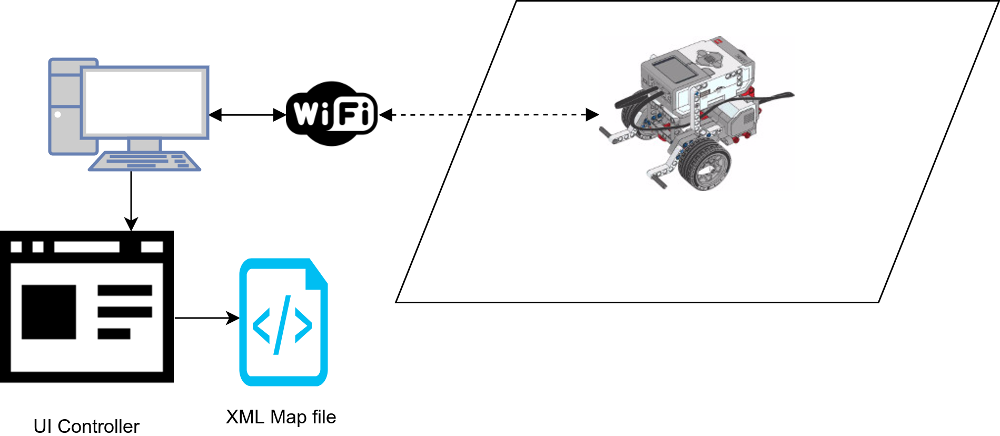
\includegraphics[width=0.9\textwidth]{Robot_system.png}
	\caption{\label{fig:robotSystem} Architectural Overview}
\end{figure}

\subsection{Component Decomposition Description}
The system has been broken down into clearly defined components, which can be tested individually. Each of these components perform a function in the entire system.

\begin{table}[H]
\centering
\begin{tabular}{|c|l|}
	\hline
	\bf{Location} & \bf{Description} \\
	\hline
	\hline
	Ev3 Robot & Embedded control software \\
	\hline
	PC & UI display \\
	\hline
	PC & Robot Control Services \\
	\hline
	PC & Robot State Logic \\
	\hline
\end{tabular}
\caption{\label{fig:compHigh}High Level Component Overview}
\end{table}

\subsection{Detailed Components Design Description}\label{detailedSection}
The following sections show the detailed design of each of the components in the system. It shows the Purpose, Function, Subordinates, Dependencies, Interfaces and Data that are required for the component.

\subsubsection{C00 Lejos Library}\label{compLejos}
\begin{itemize}
	\item Purpose: UR01,UR08,UR09,UR10,UR11,UR12,UR13
	\item Function: To interface to the robot. 
	\item Subordinates: \nameref{compMove}, \nameref{compSense} 
	\item Dependencies: Null
	\item Interfaces:
	\begin{itemize}
		\item \texttt{\detokenize{In >> ArcMoveController}}
		\item \texttt{\detokenize{Out << Ev3Remote}}
		\item \texttt{\detokenize{Out << Pose}}
		\item \texttt{\detokenize{Out << RMISampleProvider}}
	\end{itemize}
	\item Data:
\end{itemize}

\subsubsection{C01 Movement Service} \label{compMove}
\begin{itemize}
	\item Purpose: UR01,UR12,UR13,UR15,UR02
	\item Function: To provide a simple abstraction to move the robot.
	\item Subordinates: \nameref{compState}
	\item Dependencies: \nameref{compLejos}
	\item Interfaces:
	\begin{itemize}
		\item Out: \texttt{\detokenize{LocationState >> location data}}
		\item In: \texttt{\detokenize{LejosLibrary << lejos functions}}
		\item In: \texttt{\detokenize{MovementThread << Move commands}}
	\end{itemize}
	\item Data: LocationState
\end{itemize}

\subsubsection{C02 Sensors Service} \label{compSense}
\begin{itemize}
	\item Purpose: UR08,UR09,UR10,UR11,UR02
	\item Function: To provide a simple abstraction to receive sensor readings from the robot. 
	\item Subordinates: \nameref{compState}
	\item Dependencies: \nameref{compLejos}, \nameref{compShared}
	\item Interfaces:
	\begin{itemize}
		\item Out: \texttt{\detokenize{SensorsState << sensor readings}}
		\item In: \texttt{\detokenize{LejosLibrary >> lejos functions}}
	\end{itemize}
	\item Data: SensorsState
\end{itemize}

\subsubsection{C03 Robot State Machine} \label{compState}
\begin{itemize}
	\item Purpose: UR03,UR08,UR09,UR10,UR11
	\item Function: A location to define the logic what the robot does in the system.
	\item Subordinates: \nameref{compUI}
	\item Dependencies: \nameref{compShared}, \nameref{compMove}, \nameref{compSense}
	\item Interfaces:
	\begin{itemize}
		\item In: \texttt{\detokenize{SensorsState >> input into statemachine}}
		\item In: \texttt{\detokenize{LocationState >> input into statemachine}}
	\end{itemize}
	\item Data: Null
\end{itemize}

\subsubsection{C04 Shared Core} \label{compShared}
\begin{itemize}
	\item Purpose: UR03,UR14
	\item Function: This is a component to share interfaces between other components, like models and service instances.
	\item Subordinates: \nameref{compState}, \nameref{compUI}, \nameref{compSense}, \nameref{compUIUpdater}, \nameref{compMove}
	\item Dependencies: Null
	\item Interfaces:
	\begin{itemize}
		\item Out: \texttt{\detokenize{StateRepository >> output state for other parts of system}}
		\item Out: \texttt{\detokenize{ServiceManager >> output service instances for other parts of system}}
	\end{itemize}
	\item Data:
	\begin{itemize}
		\item MapPoint: shared class to represent a point on the map
		\item Colour: shared class to represent a colour on the map
	\end{itemize}
\end{itemize}

\subsubsection{C05 User Interface} \label{compUI}
\begin{itemize}
	\item Purpose: UR03,UR04,UR07,UR05,UR06
	\item Function: To provide an interactive display of the system to the user. 
	\item Subordinates: \nameref{compUIUpdater}
	\item Dependencies: \nameref{compState}, \nameref{compShared}
	\item Interfaces:
	\begin{itemize}
		\item In: \texttt{\detokenize{User interaction << Mouse clicks, key presses, handled in UI code-behind.}}
		\item Out: \texttt{\detokenize{CommandEvents >> commands to be handled by Robot State Machine}}
		\item Out: \texttt{\detokenize{MapEvents >> commands to be handled by UIUpdater}}
	\end{itemize}
	\item Data:
	\begin{itemize}
		\item MapPoint: shared class to represent a point on the map
		\item Colour: shared class to represent a colour on the map
	\end{itemize}
\end{itemize}

\subsubsection{C06 UI Updater} \label{compUIUpdater}
\begin{itemize}
	\item Purpose: UR02,UR03,UR04,UR07,UR05,UR06
	\item Function: To constantly update parts of the GUI in real time. 
	\item Subordinates:
	\item Dependencies: \nameref{compUI}, \nameref{compState}, \nameref{compShared}
	\item Interfaces:
	\begin{itemize}
		\item In: \texttt{\detokenize{UiComponent >> Allows the UIUpdater to manipulate it}}
		\item Out: \texttt{\detokenize{UiComponent << After the UIUpdater has finished making the relevant updates}}
	\end{itemize}
	\item Data:
	\begin{itemize}
		\item MapPoint: shared class to represent a point on the map
		\item Colour: shared class to represent a colour on the map
	\end{itemize}
\end{itemize}

\subsection{Architectural Alternatives}
There are several other architectural alternatives to the one that was chosen for this system. 

\subsubsection*{Single Threaded Event Loop}
A viable alternative is the single threaded event loop. In this architecture, the event loop would be continually running and functions would be called periodically based on events. This would be an efficient system, however it is important that every call is non-blocking which is hard to implement and maintain in practice, it's for this reason that a multi-threaded system was desired.

\subsubsection*{Monolithic System}
Another alternative is to combine the system code into large files. This actually reduces the amount of overall code in the system, however the code becomes hard to maintain as the code is highly interdependent. This is one of the main reasons we decided to break apart the system into multiple services.

\subsection{Design Rationale}
The system design emerged from iterative design and testing during the initial stages of the project. The rationale behind the system design can be explained by illustrating the different stages of the project.

\subsubsection{Initial Testing}
During the beginning of the system's design the architecture was very fragile, as different parts of the system were being explored in order to determine which components were necessary. It was found that several parts of the system would need to be running concurrently. The required threads are shown in Table \ref{designInit}.

\begin{table}[H]
\begin{tabular}{>{\bfseries}r l}
	SensorsThread & Fetching the sensor information \\
	MovementThread & Moving the robot, tracking location \\
	LogicThread & Handling state changes and movement subroutines \\
	GUI & Interface for users to interact with the system \\
\end{tabular}
\caption{\label{designInit}The required threads determined through testing}
\end{table}

\subsubsection{Component Development}
In this phase, the system was divided into logical components which had specific purposes. This allowed us to work on parts of the project independently in order to maximise project efficiency. The components that were defined also include the implementations for the threads determined in the initial testing stage. They are outlined in detail in section \ref{detailedSection}.

\subsubsection{Dependency Minimisation}
This was a crucial phase of system development, where the dependencies of each of the components were minimised and centralised, so that each of the components could be revised independently. This provided the system with clearly defined minimal components, which also provided easier abstractions for testing, as dependencies were minimised.
